\cleardoublepage
\chapter{Estado del arte}


En este capítulo se describen las tecnologías utilizadas para la realización de la aplicación.

\section{OTRAS HERRAMIENTAS UTILIZADAS} 
\label{sec:otras_herramientas}

El desarrollo de este proyecto se ha realizado eminentemente desde y para sistemas Linux, y concretamente se ha desarrollado y probado en distribuciones Ubuntu y Linux Mint, semejantes a los entornos que emplean profesores y alumnos en el contexto tratado.

No obstante, dado que Python es un lenguaje soportado por otros sistemas, y que en la iteración más reciente del desarrollo del proyecto se ha tendido a emplear las utilidades a través de librerías o APIs Python, o son herramientas con versión en otros sistemas. En un gran porcentaje sería portable este proyecto a otros sistemas como Windows.

En todo caso, inicialmente el desarrollo no esta considerado para otros sistemas, y exigiría la revisión de la totalidad de las dependencias de las librerías utilizadas. También sería necesaria la revisión y refactorización de algunos códigos, como por ejemplo  aquellos que emplean la librerías estándar \textit{os} y \textit{os.path}, para asegurar la plena independencia del código frente al sistema operativo.\\


Una vez circunscritos a estos sistemas, hay que recalcar que en general se ha intentado optar por el uso de editores, herramientas, librerías, DBMS de software libre, open source o en todo caso amigables con sus filosofías o licencias compatibles.\\


Aún así, durante el transcurso del proyecto, pasé a utilizar como IDE la herramienta Pycharm, que es privativa en su versión profesional, aunque contando con licencias especiales para proyectos de open source, y una versión básica con licencia no privativa.\\


En este caso, el cambio a este IDE viene justificado con una notable mejora de productividad ayudando a manejar la cantidad creciente de código, las ayudas y atajos para recordar y acceder a todas las librerías y APIs que he ido integrando, una gran ayuda en la detección de errores y \textit{warnings} previos a la ejecución, y en ejecución gracias a un potente debugger.\\


Una vez ya han sido introducidas con anterioridad las tecnologías, herramientas y librerías clave, paso a hacer una mención de dos de las herramientas que he conocido durante la realización de este proyecto, y que han sido de notable ayuda para su realización.\\

\subsection{PYCHARM}
\label{subsec:pycharm}

Como ya se ha introducido, PyCharm es un IDE multiplataforma orientado al lenguaje Python, y también al desarrollo de JavaScript y soporte para frameworks basados en estos lenguajes cono AngularJS o Django.\\


Pycharm aporta además, entre otras funcionalidades:\\

\begin{itemize}
\item Ayuda y análisis de código: autocompletado, marcado de sintaxis y errores.\\

\item Navegación avanzada entre los elementos del proyecto y del código.\\

\item Refactorización del código Python.\\

\item Depurador integrado.

\item Integración para test unitarios en Python.\\

\item Integración con sistemas de control de versiones: Git, Mercurial, Subversión, CVS.\\

\item Extensiones y disponibilidad de una numerosa biblioteca para infinidad de propósitos.\\

\item También permite la integración de herramientas externas. Por ejemplo, en nuestro caso integramos \textit{pep8} y pudiéndose chequear el estilo de cualquier módulo rápidamente.
\end{itemize}


\begin{figure}[H]
   \centering
   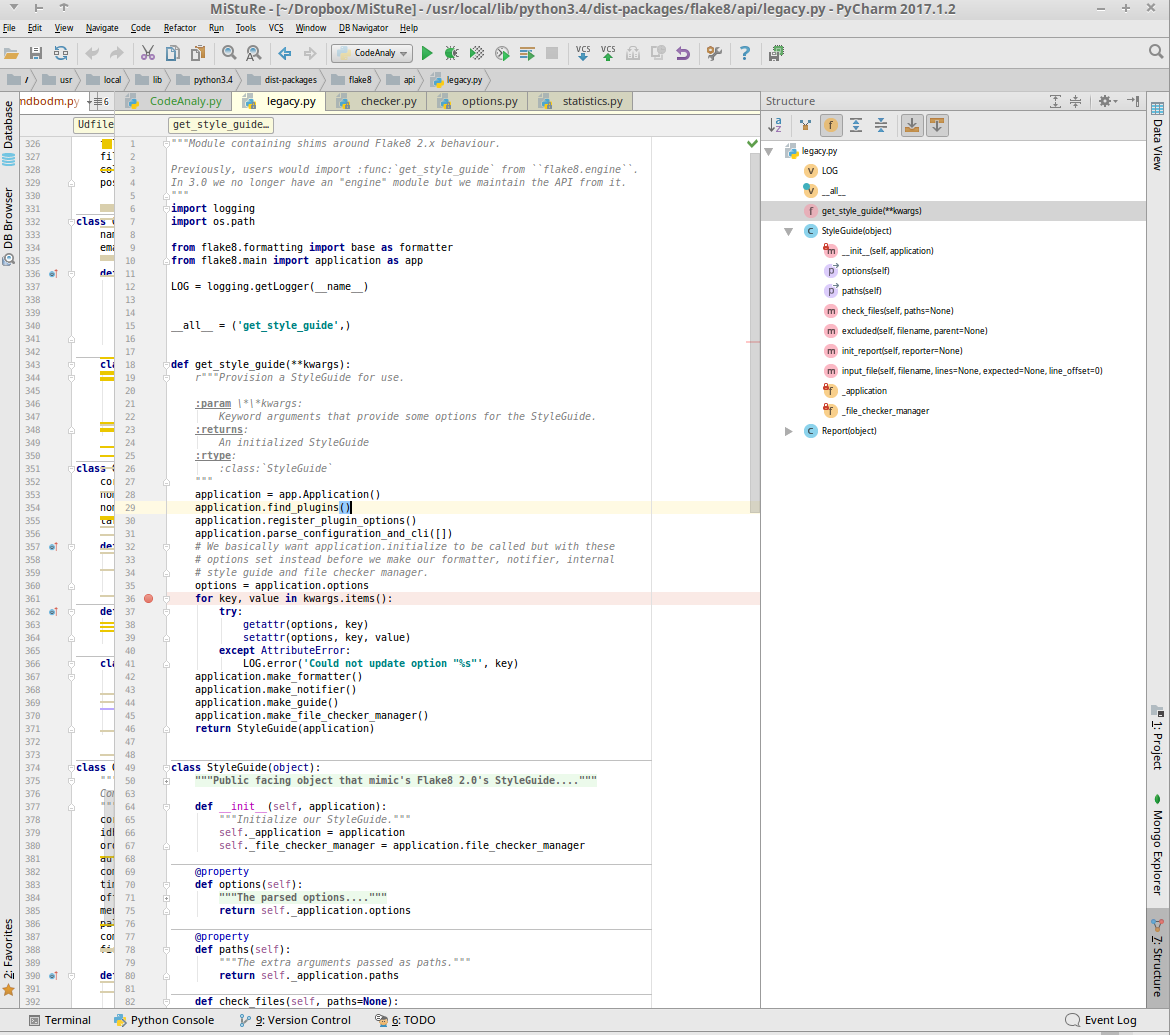
\includegraphics[width=16cm]{img/pycharm}
   \caption{Interfaz de PyCharm }
   \label{figura:pycharm}
\end{figure}



Jetbrains, la empresa desarrolladora de este producto, lo pone a disposición de los usuarios bajo un modelo que puede considerarse \textit{fremium}. Tienen disponible una versión profesional, privativa, con todas las funcionalidades y extensiones.\\


No obstante, proporcionan licencias especiales para proyectos open source no comerciales, cuyas condiciones podemos encontrar en \url{https://www.jetbrains.com/buy/opensource/}.\\


Asimismo, mantienen versiones básicas de sus productos lanzadas bajo licencias open source, como Apache 2.0, llegando a disponerse públicamente del código de algunos de ellos. Tal como es el caso de IntelliJ IDEA \url{https://github.com/JetBrains/intellij-community}, que es otro IDE desarrollado por ellos que es la propia base del IDE PyCharm.\\


En el caso de PyCharm, está versión es la denominada como ``Community Edition'', la cuál fue la que se empleo en el desarrollo y depuración de buena parte de este proyecto.\\


\subsection{ROBOMONGO}
\label{subsec:robomongo}

Robomongo es un cliente para bases de datos MongoDB con interfaz gráfica, muy ligero y de funcionalidad básica, pero suficientemente potente.\\


Además de integrar la funcionalidad del cliente shell de MongoDB, permite la escritura de scripts para mongo y la visualización rápida de las diferentes BBDD MongoDB de la conexión sobre la que se establece, asimismo de las principales características, configuraciones y contenidos de colecciones y documentos.\\


Una característica simple pero que resulta de gran ayuda, es la rapidez de navegación entre las diferentes colecciones y documentos y la posibilidad de visualización de estos en diferentes formatos como tabla, árbol, o la tradicional vista de texto en formato JSON.\\


\begin{figure}[H]
   \centering
   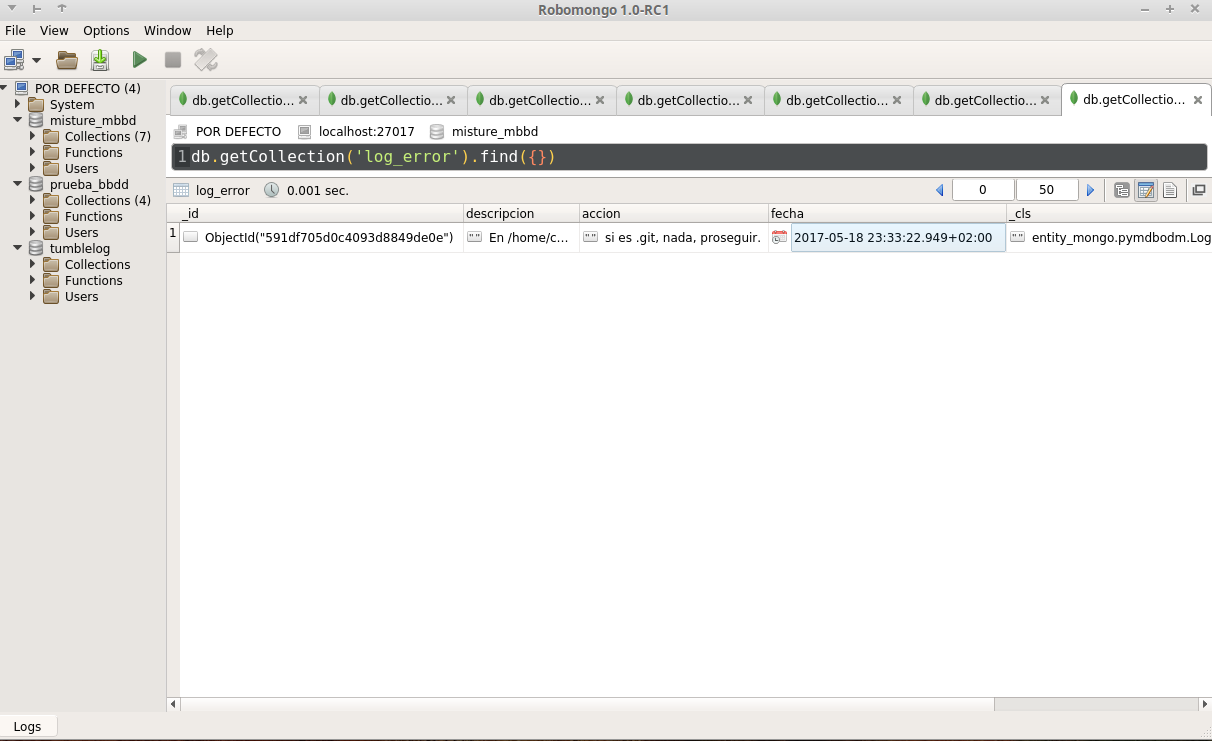
\includegraphics[width=16cm]{img/robomongo}
   \caption{Interfaz de Robomongo}
   \label{figura:robomongo}
\end{figure}


Robomongo ha estado siendo un proyecto open source cuyo código ha estado disponible públicamente. Recientemente, ha sido adquirido por la empresa Studio3T, que ha optado por mantener el proyecto en  open source \url{https://github.com/Studio3T/robomongo}, en paralelo a sus proyectos comerciales relativos a MongoDB.
